\documentclass[12pt,halfline,a4paper,]{ouparticle}

% Packages I think are necessary for basic Rmarkdown functionality
\usepackage{hyperref}
\usepackage{graphicx}
\usepackage{listings}
\usepackage{color}
\usepackage{fancyvrb}
\usepackage{framed}

% For knitr::kable functionality
\usepackage{booktabs}
\usepackage{longtable}

%% To allow better options for figure placement
%\usepackage{float}

% Packages that are supposedly required by OUP sty file
\usepackage{amssymb, amsmath, geometry, amsfonts, verbatim, endnotes, setspace}

% For code highlighting I think
\DefineVerbatimEnvironment{Highlighting}{Verbatim}{commandchars=\\\{\}}
\definecolor{shadecolor}{RGB}{248,248,248}
\newenvironment{Shaded}{\begin{snugshade}}{\end{snugshade}}
\newcommand{\AlertTok}[1]{\textcolor[rgb]{0.94,0.16,0.16}{#1}}
\newcommand{\AnnotationTok}[1]{\textcolor[rgb]{0.56,0.35,0.01}{\textbf{\textit{#1}}}}
\newcommand{\AttributeTok}[1]{\textcolor[rgb]{0.77,0.63,0.00}{#1}}
\newcommand{\BaseNTok}[1]{\textcolor[rgb]{0.00,0.00,0.81}{#1}}
\newcommand{\BuiltInTok}[1]{#1}
\newcommand{\CharTok}[1]{\textcolor[rgb]{0.31,0.60,0.02}{#1}}
\newcommand{\CommentTok}[1]{\textcolor[rgb]{0.56,0.35,0.01}{\textit{#1}}}
\newcommand{\CommentVarTok}[1]{\textcolor[rgb]{0.56,0.35,0.01}{\textbf{\textit{#1}}}}
\newcommand{\ConstantTok}[1]{\textcolor[rgb]{0.00,0.00,0.00}{#1}}
\newcommand{\ControlFlowTok}[1]{\textcolor[rgb]{0.13,0.29,0.53}{\textbf{#1}}}
\newcommand{\DataTypeTok}[1]{\textcolor[rgb]{0.13,0.29,0.53}{#1}}
\newcommand{\DecValTok}[1]{\textcolor[rgb]{0.00,0.00,0.81}{#1}}
\newcommand{\DocumentationTok}[1]{\textcolor[rgb]{0.56,0.35,0.01}{\textbf{\textit{#1}}}}
\newcommand{\ErrorTok}[1]{\textcolor[rgb]{0.64,0.00,0.00}{\textbf{#1}}}
\newcommand{\ExtensionTok}[1]{#1}
\newcommand{\FloatTok}[1]{\textcolor[rgb]{0.00,0.00,0.81}{#1}}
\newcommand{\FunctionTok}[1]{\textcolor[rgb]{0.00,0.00,0.00}{#1}}
\newcommand{\ImportTok}[1]{#1}
\newcommand{\InformationTok}[1]{\textcolor[rgb]{0.56,0.35,0.01}{\textbf{\textit{#1}}}}
\newcommand{\KeywordTok}[1]{\textcolor[rgb]{0.13,0.29,0.53}{\textbf{#1}}}
\newcommand{\NormalTok}[1]{#1}
\newcommand{\OperatorTok}[1]{\textcolor[rgb]{0.81,0.36,0.00}{\textbf{#1}}}
\newcommand{\OtherTok}[1]{\textcolor[rgb]{0.56,0.35,0.01}{#1}}
\newcommand{\PreprocessorTok}[1]{\textcolor[rgb]{0.56,0.35,0.01}{\textit{#1}}}
\newcommand{\RegionMarkerTok}[1]{#1}
\newcommand{\SpecialCharTok}[1]{\textcolor[rgb]{0.00,0.00,0.00}{#1}}
\newcommand{\SpecialStringTok}[1]{\textcolor[rgb]{0.31,0.60,0.02}{#1}}
\newcommand{\StringTok}[1]{\textcolor[rgb]{0.31,0.60,0.02}{#1}}
\newcommand{\VariableTok}[1]{\textcolor[rgb]{0.00,0.00,0.00}{#1}}
\newcommand{\VerbatimStringTok}[1]{\textcolor[rgb]{0.31,0.60,0.02}{#1}}
\newcommand{\WarningTok}[1]{\textcolor[rgb]{0.56,0.35,0.01}{\textbf{\textit{#1}}}}

% For making Rmarkdown lists
\providecommand{\tightlist}{%
  \setlength{\itemsep}{0pt}\setlength{\parskip}{0pt}}

% Part for setting citation format package: natbib

% Part for setting citation format package: biblatex

% Part for indenting CSL refs
% Pandoc citation processing
% Pandoc header

\begin{document}

\title{POLS 7012 Final Exam Practice}

\author{%
\name{YOUR NAME HERE}\address{University of Georgia}\email{\href{mailto:email@email.email}{email@email.email}}
\and
\name{Joseph T. Ornstein}\address{University of Georgia}\email{\href{mailto:jornstein@uga.edu}{jornstein@uga.edu}}
}

\abstract{In this practice final exam, we will replicate some results from ``Local
demographic changes and US presidential voting, 2012 to 2016'' (Hill,
Hopkins, and Huber 2019). You can find the paper in the \texttt{papers/}
folder, and the data you'll need in (you guessed it) the \texttt{data/}
folder. Write you code in the chunks provided, then knit the document to
a PDF.}

\date{December 08, 2020}

\keywords{}

\maketitle



\hypertarget{introduction}{%
\section{Introduction}\label{introduction}}

Hill, Hopkins, and Huber (2019) investigate whether support for
Republican candidates in US presidential elections is correlated with
demographic changes at the precinct level. They find, contrary to their
expectations, that precinct-level increases in the Hispanic share of a
population are not significantly associated with shifts in vote share
from Obama in 2012 to Trump in 2016. Before you begin the replication,
skim over the paper a bit. We'll be replicating Figure 1 and Table 1.
Follow the instructions below, and for an extra challenge, you can
complete any steps listed as ``an extra challenge''.

\hypertarget{data}{%
\section{Data}\label{data}}

The precinct-level data is a Stata file called ``PrecinctData.dta''. I
downloaded it
\href{https://dataverse.harvard.edu/dataset.xhtml?persistentId=doi:10.7910/DVN/J5GCZQ}{here}.
Start by reading the data file into memory. Consult the codebook for
variable definitions.

\hypertarget{results}{%
\section{Results}\label{results}}

\hypertarget{replicating-figure-1}{%
\subsection{Replicating Figure 1}\label{replicating-figure-1}}

Figure 1 plots the relationship between changes in Hispanic population
and changes in Republican vote share for a subset of the precincts,
along with a fitted LOESS curve (Locally Estimated Scatterplot
Smoothing; the default in \texttt{geom\_smooth()}). To recreate this
figure, we'll need to complete the following steps:

\begin{itemize}
\tightlist
\item
  Create four plots, named \texttt{p1}, \texttt{p2}, \texttt{p3}, and
  \texttt{p4}.
\item
  Add a \texttt{geom\_point()} and \texttt{geom\_smooth()} layer to each
  plot with the appropriate variable mappings
\item
  Color the LOESS fit green
\item
  Add axis labels to the plot to match the labels from the paper
\end{itemize}

\noindent For an extra challenge, you can complete any combination of
the following:

\begin{itemize}
\tightlist
\item
  Before creating each subplot, filter the data so that it only includes
  only the interior 5\% to 95\% quantiles of the x variable. (They
  mention this step in a footnote on page 4. Sneaky sneaky.) The
  \texttt{quantile()} function is useful here.
\item
  Draw a random sample of 2,000 precincts for the scatter plot, like in
  the original figure (but keep the LOESS fit for the full dataset).
\item
  Make the points semi-transparent
\end{itemize}

The \texttt{patchwork} library helps stitch together a bunch of ggplots
into a grid, like in the original paper.\footnote{I previously showed
  you \texttt{cowplot}. That would work too, but I wanted to try
  something new here.} If you created \texttt{p1}, \texttt{p2},
\texttt{p3}, and \texttt{p4} correctly, the included code chunk will
recreate Figure 1.

\begin{figure}[p]
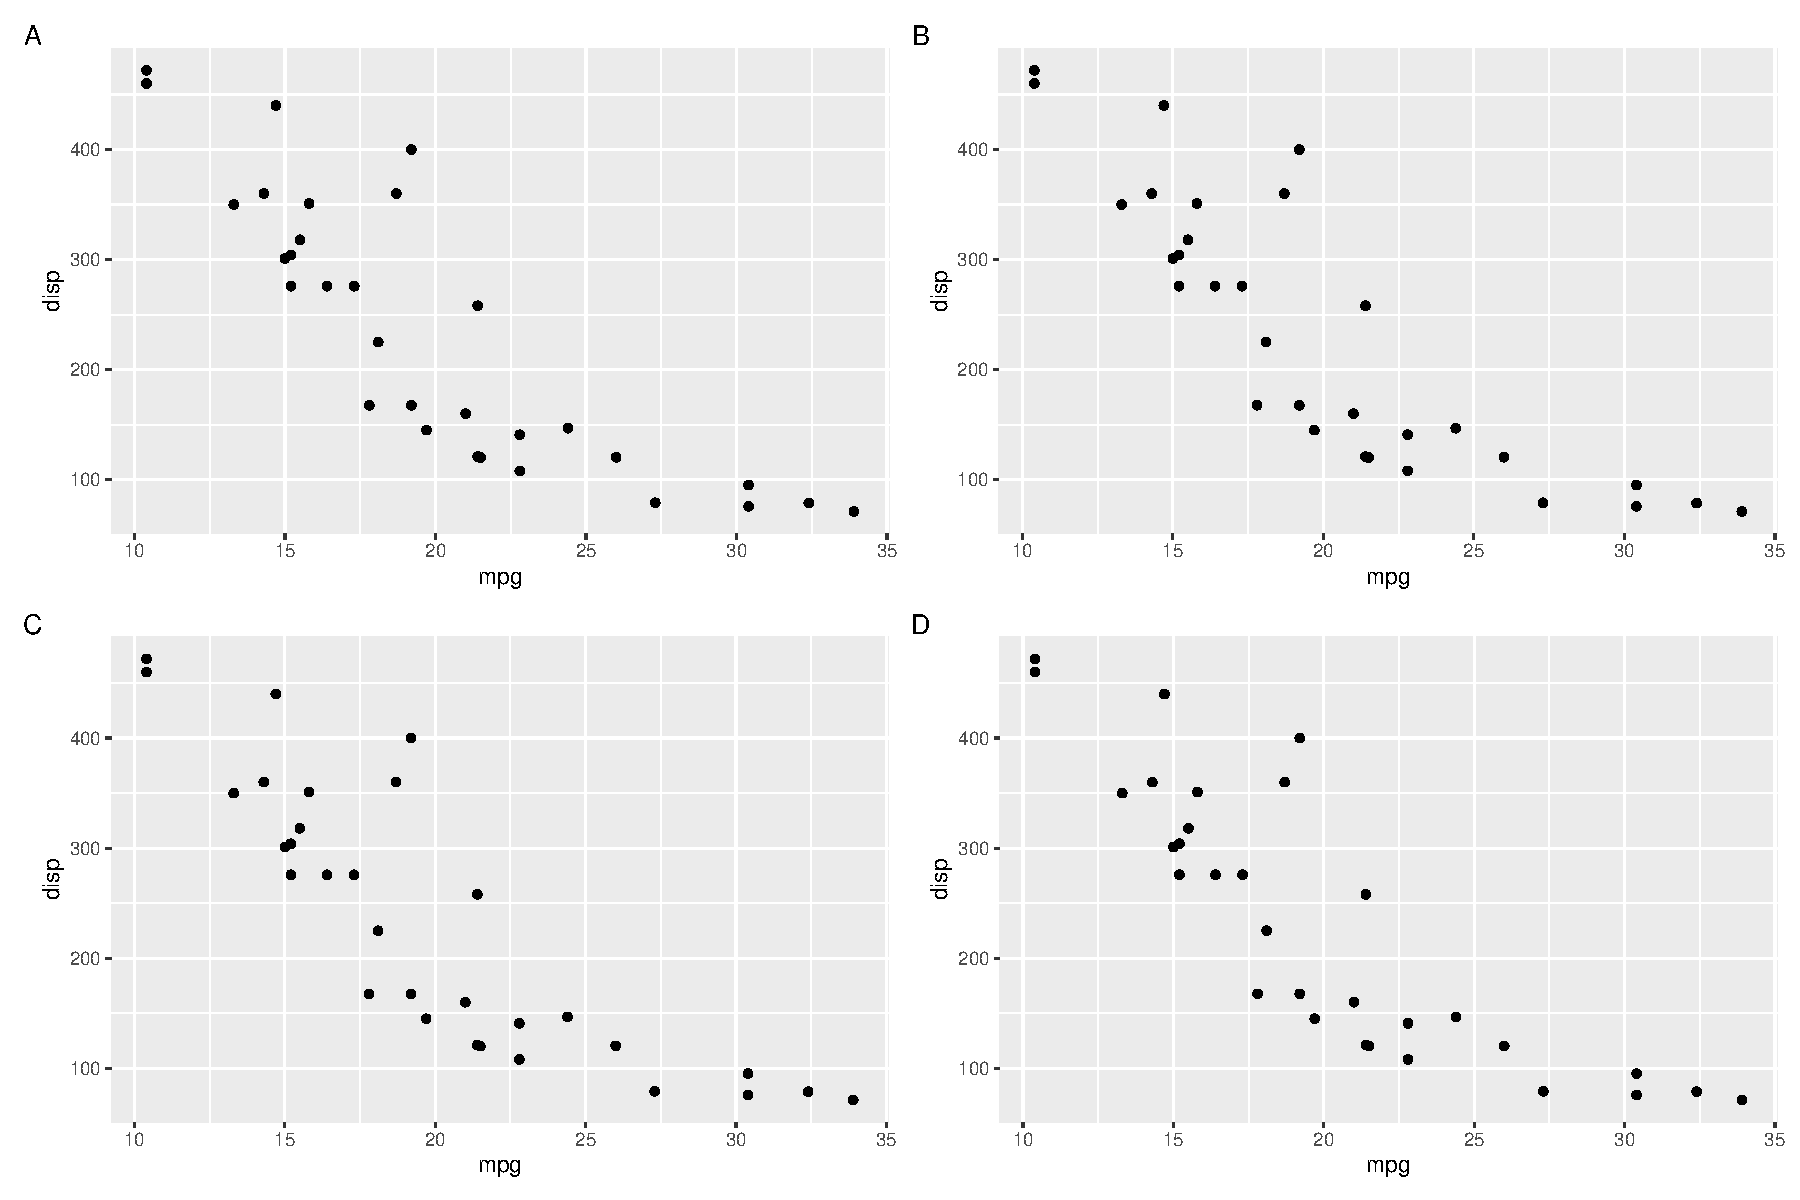
\includegraphics[width=1\linewidth]{hill-hopkins-huber_files/figure-latex/arrange plots with patchwork-1} \caption{Change in Republican vote share, 2012 to 2016, and change in Hispanic population. Note: Points are random samples of 2,000 precincts. Loess lines are generated from all observations. Points are shaded corresponding to density, with darker colors indicating more precincts.}\label{fig:arrange plots with patchwork}
\end{figure}

\hypertarget{replicating-table-1}{%
\subsection{Replicating Table 1}\label{replicating-table-1}}

In Table 1, the authors estimate a series of eight linear models to test
whether the relationships from Figure 1 remain after conditioning on
potential confounders. In each model, change in Hispanic share is
negatively associated with change in Republican vote share from 2012 to
2016. We'll replicate the first three columns of that table. To do so,
take the following steps:

\begin{itemize}
\tightlist
\item
  The first model, \texttt{lm1}, is a linear model with the change in
  GOP vote share as the outcome variable and change in the share of
  Hispanic population between 2011 and 2016 as the explanatory variable.
\item
  The second model, \texttt{lm2}, includes ``County Fixed Effects''.
  This just means including a indicator (dummy) variable for each
  county. Recode \texttt{countyid} as a character or factor and include
  it in the model.
\item
  \texttt{lm2} also includes a set of ``Additional Census Controls'' and
  ``Controls For Levels''. The full list of variables is on page 4;
  cross-reference the codebook for variable names.
\item
  The third model, \texttt{lm3}, includes all the covariates as
  \texttt{lm2}, plus a set of indicator variables measuring the
  Republican 2012 vote share decile.
\item
  Note that their models are estimated using weighted least squares
  (WLS) instead of orindary least squares (OLS). This procedure gives
  more weight to precincts with larger populations when estimating the
  best fit equation. It turns out not to matter much; you'll get pretty
  similar estimates with OLS. But to replicate their results, add the
  argument \texttt{weight\ =\ weights} to \texttt{lm()}.
\item
  Don't worry if your standard errors don't exactly match up. You'll
  learn more about ``robust'' standard errors next semester.
\end{itemize}

The following code chunk uses the \texttt{stargazer} package to output a
pretty regression table like the one in Table 1. I provide it to you
free of charge. All you need to do is make sure that the model objects
\texttt{lm1} through \texttt{lm3} are correctly specified. For an extra
challenge, you can do any combination of the following:

\begin{itemize}
\tightlist
\item
  Try to replicate columns (4) through (8).
\item
  Play with the \texttt{stargazer()} options to edit the layout and/or
  the covariate labels.
\item
  Figure out why the number of observations and coefficient estimates
  are \emph{slightly} different in \texttt{R} than the results the
  authors got from Stata. I genuinely have no idea. They may have
  copy-and-pasted wrong.
\end{itemize}

\begin{table}[!htbp] \centering 
  \caption{Change in Republican vote share 2012 to 2016 and change in Hispanic population, various time intervals} 
  \label{} 
\small 
\begin{tabular}{@{\extracolsep{1pt}}lccc} 
\\[-1.8ex]\hline 
\hline \\[-1.8ex] 
\\[-1.8ex] & (1) & (2) & (3)\\ 
\hline \\[-1.8ex] 
\hline \\[-1.8ex] 
Observations & 32 & 32 & 32 \\ 
R$^{2}$ & 0.472 & 0.472 & 0.472 \\ 
\hline 
\hline \\[-1.8ex] 
\textit{Note:}  & \multicolumn{3}{r}{$^{*}$p$<$0.05; $^{**}$p$<$0.01; $^{***}$p$<$0.001} \\ 
\end{tabular} 
\end{table}

\hypertarget{references}{%
\section*{References}\label{references}}
\addcontentsline{toc}{section}{References}

\hypertarget{refs}{}
\leavevmode\hypertarget{ref-hillDemographicChangeThreat2019}{}%
Hill, Seth, Daniel J. Hopkins, and Gregory Huber. 2019. ``Demographic
Change, Threat, and Presidential Voting: Evidence from U.S. Electoral
Precincts, 2012 to 2016.'' \emph{PNAS}, 1--6.
\url{https://doi.org/10.2139/ssrn.3351950}.






\end{document}
